\documentclass[12pt]{article}
\usepackage{candor, setspace, color, wrapfig}
\usepackage[final, colorlinks=true, linkcolor=BWFBlue,
  citecolor=BWFGreen, urlcolor=BWFRed, pdftitle={Computational
    Modelling Ribosomal Translation and Frameshifts},
  pdfauthor={Hao Lian, Vivek Bhattacharya, and Daniel Vitek},
  pdfsubject={Bioinformatics, Genetics, and Biology}, pdfcreator={The
    Frameshift Kids}, pdfkeywords={bioinformatics,genetics,biology,
    frameshifts,perl,matlab,ecoli,prfb,rpos,bgh}, pdfstartview={FitH}]{hyperref}

\linespread 2
\numberwithin{equation}{section}

\author{{\sc Hao Lian, Vivek Bhattacharya, and Daniel Vitek}}
\date{{\sc \today}}
\title{{\bf Computational Modelling Ribosomal Translation
    and Frameshifts}}

\begin{document}
\pagenumbering{roman}
\maketitle
\tableofcontents
\clearpage

\begin{abstract}
  \begin{normalsize}
  In this document, we discuss a stochastic model for ribosomal displacement relative to reading 
  frame based on forces arising from changes in free energy present in hybridization between the 
  16S rRNA tail and nucleotides upstream from the A-site.  We present both our investigation and 
  potential applications for this model, including optimization of economically significant gene
  sequences such as bovine growth hormone, non-experimental prediction of translational efficiency for man-made 
  proteins, adjustment of calculated tRNA availability values, and modelling of frameshifts in \prfB\ in \ecoli.  This
  investigation is presented as a series of sections comprising of various inquiries that were made 
  in subjects ranging throughout the field of molecular biology.  We also applied our stochastic 
  model to create a short, 16-codon sequence that is not known to produce a frameshift in nature 
  in order to test our model's predictive power for synthesized mRNA sequences, and designed an 
  experiment to verify this frameshift.  Results are expected at the beginning of October 2007.
  \end{normalsize}
\end{abstract}

\clearpage

\pagenumbering{arabic}
\section{Introduction}

Since the advent of gene sequencing technology, bacteria---in particular,
\emph{Escherichia coli}---have been studied as potential factories for the
mass production of synthetic proteins.  The optimization of the production
of human insulin in \ecoli\ epitomizes the utility of this idea.  Yet, the
intricate details of protein translation are not fully understood; differentiating
between a high-yield and a low-yield sequence often requires tedious and costly
biological experimentation.  

To attack this problem, we propose a stochastic model for translation in the 
ribosome.  We study the applications of this model as a means of screening for 
high-yield proteins without biological experimentation.  In addition, we analyze 
the applications of this model in the detection of ribosomal frameshifts.

\subsection{Protein Translation}

A cell's genetic material resides within its DNA, a long string
of nucleotides containing one of four nitrogenous bases: adenine,
guanine, cytosine, and thymine.  However, DNA is not
directly involved in the process of producing a protein.  Rather, through
a process called \emph{transcription}, the cell produces messenger RNA from DNA.
This mRNA then arrives at a ribosome and undergoes ribosomal \emph{translation}, or
protein production.

Each group of three nucleotides on the mRNA strand forms a \emph{codon}.
Each codon, furthermore, codes for a specific amino acid.  When the mRNA
is in the ribosome, transfer RNA molecules bring amino acids
to the ribosome.  Once the proper amino acid is found for the current codon,
the ribosome shifts three nucleotides in view---one full codon---and waits
for a tRNA to bring the appropriate amino acid.  In turn, these amino acids
bond together to form the full protein.

\section{Description of the Model}
\label{allmodel}

\subsection{Free Energy}
\label{freeenergy}

Free energy in a cell arises from the hybridization between two
sequences of RNA and drives ribosomal translation~\cite{starmer}.
\citet{weiss88} suggest the 16S tail of the ribosome hybridizes with its mRNA strand;
from this, we can calculate the free energy values for the interaction between the two strands of RNA.
\citet{freier} propose a thermodynamic model for exactly this,
modeling the interaction in terms of \emph{doublets}, which are pairs of consecutive nucleotides.
Using this model, Freier calculated the free energy available
for the hybridization of permutations of RNA doublets.

\subsection{A Deterministic Model for Displacement} 
 
\citet{lalit:mechanics} assume a sinusoidal model for
free energy, whence we can project free energy onto magnitude and
phase through a memory model. Ponnala simulates free
energy in a memory structure that can store three values (registers)
that he later can represent as a phasor, a concept from physics. Then,
we can visualize free energy from polar plots and deduce frameshifts,
which occur along defined boundaries~\citet{lalit:mechanics} on the polar plot for a species.
 
\citet{lalit:embs} then represent the cumulative phasor
at codon $k$ as $\bvec{V} = Me^{i\theta}$ where $i$ is the imaginary
constant, allowing us to calculate the magnitude and phase at codon
$k$ through simple trigonometry. Magnitude and phase are then modeled
as a polar plot, one of the model outputs. Differentiating this vector, we
arrive at vector $\bvec{D}$ for instantaneous energy, interpreting
this as a force that acts on the ribosome, keeping the mRNA in
a given reading frame.
 
The length of time that the force acts on the ribosome depends upon
the codon's tRNA availability at the A-site during translation.
\citeauthor{lalit:mechanics} use a deterministic model to represent this: For each codon,
a number of ``wait cycles," dependent upon the rarity of the
associated tRNA, correspond to the number of times the force can
increment displacement from the current reading frame.  In the
deterministic model, the force acts for \emph{exactly} this set number
of cycles given a codon. We can then simulate hybridization between the
16S ribosomal subunit and a given mRNA strand: First, the 13-base 16S
tail of \ecoli\ hybridizes with the first 13 bases of a sequence,
which is a 12-base leader sequence and the first base of the start
codon \textsc{aug}, to determine the free energy value of the first acid.
Then, shifting one base pair at a time, we calculate the free energy
for the entire sequence according to \citet{starmer}.

\subsection{Frameshifts}
\label{section:frameshifts}

\begin{figure}
  \centering
  \caption{Deterministic displacement plot of~\prfB}
  \label{prfB:deterministic}
  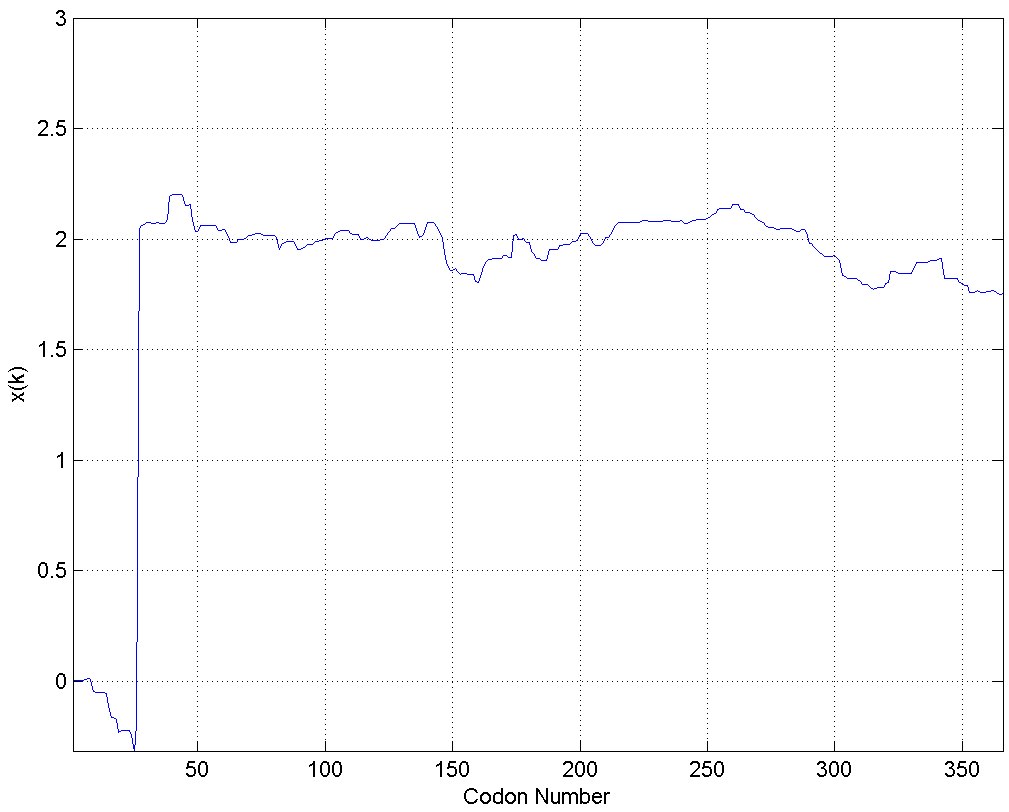
\includegraphics[scale=0.4]{prfB/deterministic}
\end{figure}

\begin{wrapfigure}{R}{0.5\textwidth}
  \centering
  \caption{Polar plot of \prfB}
  \label{prfB:polar}
  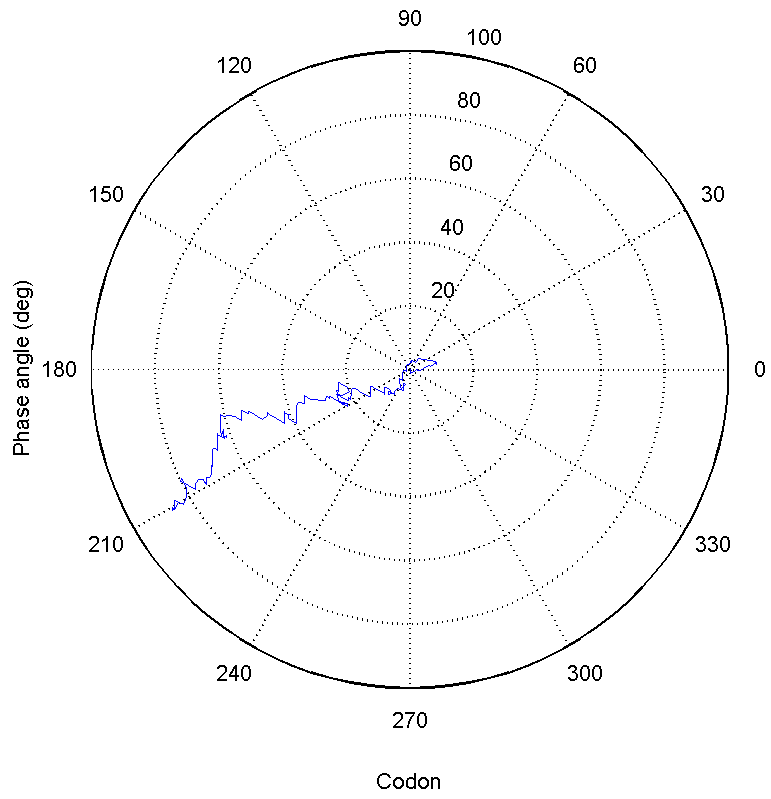
\includegraphics[scale=0.5]{prfB/polar}
\end{wrapfigure}

First, we let a displacement of $x = 0$ correspond to the zero reading frame and increments of
\emph{two} to represent a one-nucleotide change. For example, $x =2$ represents the +1 frame.
\citet{lalit:embs} prove that both $x = 0$ and $x = 2$ are fixed (stable) points in displacement in their model,
as expected.

A sudden jump from approximately $x = 0$ to $x = 2$ is then the first indication of a $+1$ frameshift.
In essence, this jump suggests that the ribosome skips one entire base pair in the mRNA sequence.
\autoref{prfB:deterministic} shows the displacement plot per this deterministic model for \prfB, 
a gene with a programmed $+1$ frameshift at codon 25.

In conjunction with this characteristic plot, a $+1$ frameshift also displays a clockwise 120\degree\
phase angle rotation from the species angle, consistent with the
creation of the displacement vector from the phasors.
Intuitively, a frameshift sustains if the free energy signal aligns with the sudden jump in displacement.
Since the free energy signal has a period of one codon~\cite{lalit:mechanics}, a $+1$ frameshift the free energy signal
must undergo a phase shift of one-third of an entire period (\autoref{prfB:polar}).

\subsection{A Stochastic Model for Displacement}
\label{stochastic}

As mentioned, the gene \prfB\ exhibits a definite frameshift under the
deterministic model: The displacement jumps to $x=2$.  Certain other
genes, however, demonstrate equivocal, ambiguous behavior near $x = \pm
1$~\cite{lalit:embs}.  In a deterministic model, the fixed
displacement plots implies we cannot clearly interpret whether this
behavior indicates a tendency for a stable frameshift. Even worse,
the model may not show these unstable behaviors at all. In practice,
ribosomal translations are not deterministic. Due to the presence of
noise within the cell environment, we instead chose to model
translation stochastically, adding randomness to the choice of reading
frame a ribosome performs at each codon based upon the free energy signal.
As such, we introduce probability into the model.

We propose that at each cycle in elongation, the ribosome must make a
decision: stay in the current reading frame, move to the $+1$ reading
frame, or move to the $-1$ reading frame.  We can further subdivide
this choice into the individual wait-cycles.  At each wait cycle, the
ribosome chooses from the above possibilities or proceeds to another
wait-cycle without making a decision.

Let $abcd$ be a sequence of four nucleotides, with $abc$ in the
current reading frame and $bcd$ in a +1 reading frame.  Let $x$ be the
displacement of the current wait cycle of the ribosome.  As the
incremental displacement approaches +1, the probability of choosing
codon $bcd$ should increase and the probability of choosing codon
$abc$ should decrease.  We model this behavior using even powers of
cosine and sine functions for $abc$ and $bcd$.  We
define $\omega$ as the \emph{weight} that is directly proportional to
the probability.
\begin{equation}
  \omega_{abc} = \cos^{10}{\frac{x\pi}{4}} \text{ and } \omega_{bcd} =
  \sin^{10}{\frac{x\pi}{4}}.
  \footnote{For the purposes of this model, the cosine and sine
    functions are taken to the tenth power, but in future studies,
    this parameter, which must be an even integer, can change.}
\end{equation}
If the ribosome lies completely in the 0 frame, then the probability
of staying in the 0 frame should be 1.  Consequently, if the ribosome
lies fully in the +1 frame ($x=2$), the probability of going to the 0
frame should be 0. Therefore, these functions have a period of two
base pairs ($x=4$).

Now we define a value $n_{abc}$ based upon normalizing $N_{abc}$, the
number of wait cycles, itself inversely proportional to the
tRNA availability of codon $abc$.
We want to wait long enough that the probability of assume the probability of frameshifting after
after $N_{abc}$ wait cycles is $\frac{1}{2}$.  Let $P$ be the
probability of moving on to the next codon and staying in current reading
frame.  Then we should have $1-\left(1-P\right)^{N_{abc}} =
\frac{1}{2}$.

Now assume we are at a particular wait cycle. In absence of further
research, we assume by the principle of indifference the probability
of frameshifting is 1/2.  Let $P$ be the instantaneous probability of
moving on to the next codon and staying in the current reading frame.
Then we should have $1-\left(1-P\right)^{N_{abc}} = \frac{1}{2}$.
Given that $P \propto \omega_{abc}$, let $n_{abc}$ be the constant of
proportionality; thus $n_{abc} = \omega_{abc} / P$.  We have
$\omega_{abc} \le 1$, so hence $n \le \sqrt[N]{2}/(\sqrt[N]{2} - 1)$
where $n = n_{abc}$ and $N = N_{abc}$.  Mathematically, the
probability of choosing the codon in the current reading frame is just
\begin{align}
  \prod_{i=1}^K \left(1-\frac{\omega_i}{n}\right) \text{ where } \omega_i = \cos^{10}{\frac{x_i\pi}{4}}.
\end{align}
Here, $n$ represents the wait time for that codon and $K$ is the
ordinal of the wait cycle. For example, $K=1$ on the first wait
cycle, $K=2$ on the second, and so forth.  Importantly,
$\omega$ is dependent on displacement, which increments after
every wait cycle.

\subsection{Measures of Sequence Analysis}

As this model is stochastic, multiple runs (the sample size) of the same sequence must be analyzed.
As such, we propose two metrics for analysis of a number of different runs 
simultaneously. 

\subsubsection{Error-Free Rate}

When studying a
sequence with a programmed frameshift, it measures the percentage of runs 
during which the ribosome chooses the correct codon
at \emph{every} juncture.  For a +1 frameshift, for example, the ribosome must
choose the +1 frame at the frameshift codon and stay in the 0 frame before
and the +1 frame after in order for the run to be a success.

\subsubsection{Displacement Deviation}
\label{section:deviation}

We propose the formula
\begin{equation}
    \label{eqn:lbd}
    d = \sqrt{\frac{\sum_i \left(x_i - \beta_i\right)^2}{N}}
\end{equation}
where $\beta_i$ is the predicted reading frame at codon $i$, $x$ is the displacement at codon $i$,
and $N$ is the total number of codons as a measure of the deviation of the sequence
from the expected reading frame.  Usually $\beta_i = 0$ unless a
programmed frameshift exists as it does for \prfB.
For example, for \prfB\ $\beta_i = 2$ for all $i \geq 25$ because \prfB\ frameshifts at codon 25 \textsc{uga}
and the model represents a frameshift with +2 displacement per \autoref{section:frameshifts}.

\section{Calibrating tRNA Availability Values}

From \autoref{stochastic}, it becomes clear that the model depends upon
its input parameters, all of which have to be tuned to optimize
the predictive power of the model.  As will be discussed in later sections,
many of these parameters, including the species angle and the initial displacement,
are robust; minor changes in these values will have negligible repercussions
on the output of the model.  A parameter that is much more difficult to estimate
is tRNA availability value (TAV) vectors.

\citeauthor{lalit:embs} base the tRNA availability values on codon usage, 
surveying a set of genes from \ecoli.
Although this assumption has biological basis~\cite{ikemura}, 
it is possible that the true values for these numbers may differ 
due to sampling error or the choice of genes chosen.
Taking a different tack, we chose to calibrate TAV vectors from
existing biological data, designing a genetic algorithm to calibrate
these values based on the bovine growth hormone (bGH) sequences.
As discussed in \autoref{section:bgh}, \citet{schoner:bgh}
have conducted experiments that propose a set of eight sequences coding for bGH,
two of which have very high yield (pcZ101 and pcZ105) and six of which have low yield.
Since these sequences are known to be translationally regulated, they
provide an excellent method of calibration.

We optimize the separation between the yields of pcZ101 and pcZ105 and those of other bGH sequences.  
First, we generate a list of randomly modified TAV vectors at which
point we calculate the ratio of the displacement deviation from
displacement (\autoref{section:deviation}) for pcZ101 and pcZ105 to the other
six bGH proteins. From there, we sort the modified TAV according to
this ratio and discarding the least optimal half of the tRNA
vectors. We then choose two of the remaining vectors, with the chance
of each vector being proportional to its rank.  We then take a
weighted average of the two vectors and spawn a new vector.  After
creating the next generation according to a constant ``gene pool''
size, we delete the previous generation and repeat. After a fixed
number of generations, the algorithm terminates and returns the
optimal TAV vector.

This algorithm did not alter the TAV vectors to a significant degree.
In fact, the average change to each value in the vector was merely
10\%.  Yet, the newly generated vector returns much more optimal
results than values from \citeauthor{lalit:embs}.  The new values
are used throughout the remainder of the paper to produce the 
values and graphs.

\section{Translational Efficiency}

% Need citations for the following paragraph.

A central problem in modern genetics is that
although most bacteria, like \ecoli, are known to regulate protein production
on the transcriptional level, synthetic genes often encounter \emph{translational}
problems.  Microbiologists usually resort to trial-and-error to determine genes
that translate at optimal level, but we can develop a computational method
to roughly predict the translational efficiency of synthetic genes to
be run in \ecoli.

\autoref{allmodel} implies that divergence from $x=0$ causes
problems in translation, an essential characteristic
of a frameshift.  Thus, we stipulate that high translational efficiency correlates to low deviation yield,
since this requirement implies proximity to the horizontal axis.  This section
evaluates the proposed metric.

\subsection{Ribosomal Proteins}

% CITATION ???

\begin{wrapfigure}{R}{0.55\textwidth}
  \centering
  \caption{Displacement deviation for \ecoli\ genes with <1\% of genes
    with deviation >3 truncated}
  \label{ecoli:hist}
  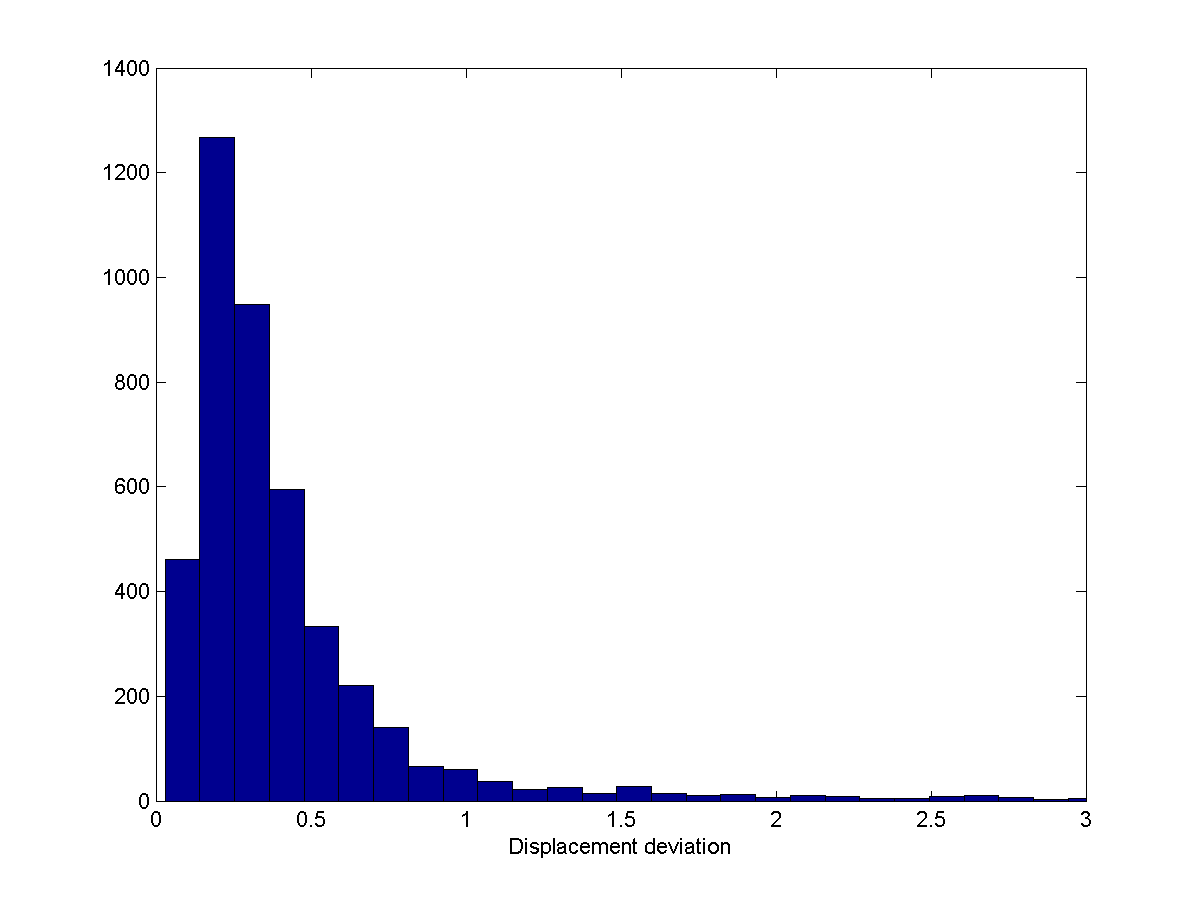
\includegraphics[width=0.55\textwidth]{histograms/everything}
\end{wrapfigure}

\ecoli, as a product of evolution, is naturally efficient in its
processes.  It logically follows that the model should indicate low deviation
for most \ecoli\ proteins.  Indeed, computational data supports this hypothesis.
\autoref{ecoli:hist} is a histogram of the deviation yields of 4364 genes of
\ecoli, over 80\% of the entire genome.  As predicted, the vast majority
of these genes lie in the 0 to 1 interval.  The average displacement deviation
for these \ecoli\ genes is 0.4483, run for 100 iterations per genes.

To compound this finding, biologists also agree that ribosomal proteins
offer especially high translational efficiencies, since the cell must produce
them in such large quantities.  The displacement deviation for ribosomal
proteins is in fact 0.2515.

\subsection{Bovine Growth Hormone}
\label{section:bgh}

% Perhaps include a plot of Schoner's yield and our deviation.

We investigated the concept of deviation yield as a measure of biological
yield by studying bovine growth hormone (bGH), a protein commonly used
in agriculture and thus possessing wide commercial benefit.
Research~\cite{schoner:bgh} at the time attempted to produce bGH
in \ecoli\ in large amounts.  As this process was purely biological, researchers
simply induced changes in a sequence until protein yield increased, thus resulting
in a rather arduous process. In contrast, our model can accurately
differentiate between high and low yield proteins, thus providing a preliminary screen
to determine translational efficiency before biological verification.

\begin{figure}
\centering
\begin{singlespace}
    \begin{tabular}{lcc}
        \toprule
        \textbf{Sequence} & $d$ & $\sigma(d)$\\
        \midrule
        pcZ101 & 0.51373 & 0.04278 \\
        pcZ105 & 0.51723 & 0.04601 \\
        \midrule
        pcZ100 & 0.69547 & 0.01576 \\
        pcZ104 & 0.69061 & 0.01976 \\
        pcZ108 & 0.64429 & 0.03941 \\
        pcZ110 & 0.69257 & 0.01776 \\
        pcZ112 & 0.67896 & 0.02403 \\
        pcZ115 & 0.68986 & 0.02028 \\
        \bottomrule
    \end{tabular}
    \caption{Deviations for bGH Sequences with Sample Size~500}
    \label{bgh:deviation}
\end{singlespace}
\end{figure}

\citet{schoner:bgh}, primarily modifying the initial codons of an initial
bovine growth hormone sequence, found two sequences pcZ101 and pcZ105
to have particularly high protein yield and to be efficient in
comparison to
the six other sequences. Our model agrees with his findings. In modeling displacement,
we found pcZ101 and pcZ105 to have the least reading frame deviation
from $x = 0$ (\autoref{bgh:deviation}). \autoref{bgh:disp} shows the displacement
plots of all the bGH sequences on the same set of axes.  The two with the highest yields
are in green and turquoise and stay close to the axis, suggesting that with the
new tRNA calibrations, low deviation may correspond to higher yield.

\begin{figure}
  \centering
  \caption{Displacement plot for bGH}
  \label{bgh:disp}
  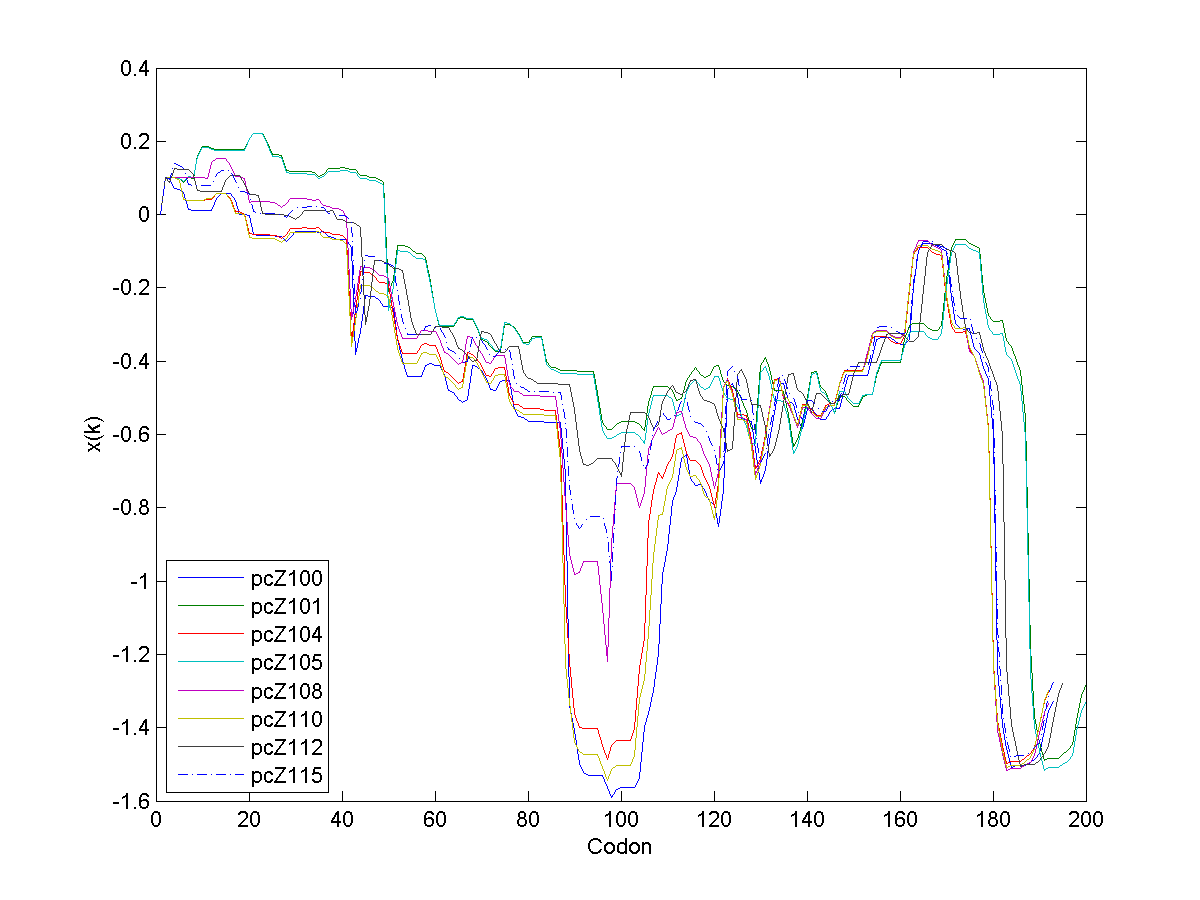
\includegraphics[scale=0.4]{bgh/all}
\end{figure}

In addition, in examining the polar plots, we noticed that during
early translation the phase of translation for pcZ101 and pcZ105 tended toward the species
angle $-30\degree$ before diverging toward approximately $15\degree$. As
it stands, our model, as with displacement, indicates higher yield when the polar plot
indicates less deviation from the correct, zero reading frame, as it
does here with the species angle~\cite{lalit:mechanics}. Therefore our
model is consistent with research that indicates
the early codons have a dramatic impact on the ultimate efficiency of
ribosomal translation.

These results from bovine growth hormone in addition to correlation with a broad
spectrum of known ribosomal behavior indicate our computational model
can significantly increase the speed at which geneticists and
biologists can obtain valuable information when synthesizing
commercially or medicinally useful compounds without laboriously
working through biological experiments.

\subsection{Optimizing Translational Efficiency}

If deviation yield is in fact a potential metric for biological yield,
a method for optimizing deviation would be of use of biologists.  As such,
we wrote an algorithm to minimize deviation for given sequences.
We tested this algorithm computationally on \rpoS, a gene known to
be translationally regulated.  Biological experiments will be
conducted soon.

% I'm colluding deviation and probability yield here, but it's for a
% good purpose. --Hao.

\citet{rpoS:process} indicate that \rpoS, a gene that codes for an RNA
polymerase sigma factor, contains sections of rare codons that disrupt
ribosomal translation. Indeed, our computation model agrees with this
biological evidence, showing again moderately high deviation from $x =
0$. In mass production of such a polymerase sigma factor, biologists
can replace sequences of codons known to add noise and error to
ribosomal translation with synonymous codons. 
However, with a computation model, the process is much
faster and, with this performance, we can perform a randomized, greedy
algorithmic search for codon sequence replacements. We first find an
early trouble spot\footnote{Specifically, places with
  mistake frameshifts in our model, which correlate to rare codons per
  above discussion.} of four codons, randomly replacing that sequence
with synonymous four codons, and running our model against those
permutations to obtain a locally optimal sequence at that place. We
then repeat for all trouble spots the first, terminating when we have locally
optimized the last one. With this algorithm, we reduced our standard
deviation metric for the \rpoS\ displacement plot from 0.168 to 0.117
on sample size of 1000 with a replacement of 33 codons. The
initial correlation between deviation and biological expression
provides strong anecdotal evidence that, with future biological
experimentation, our algorithm has indeed increased protein yield
bypassing a potentially slow biological experimentation process.

\section{Frameshifts}

\subsection{Results for \prfB}

\begin{figure}
  \centering
  \caption{Stochastic displacement plot of \prfB}
  \label{prfB}
  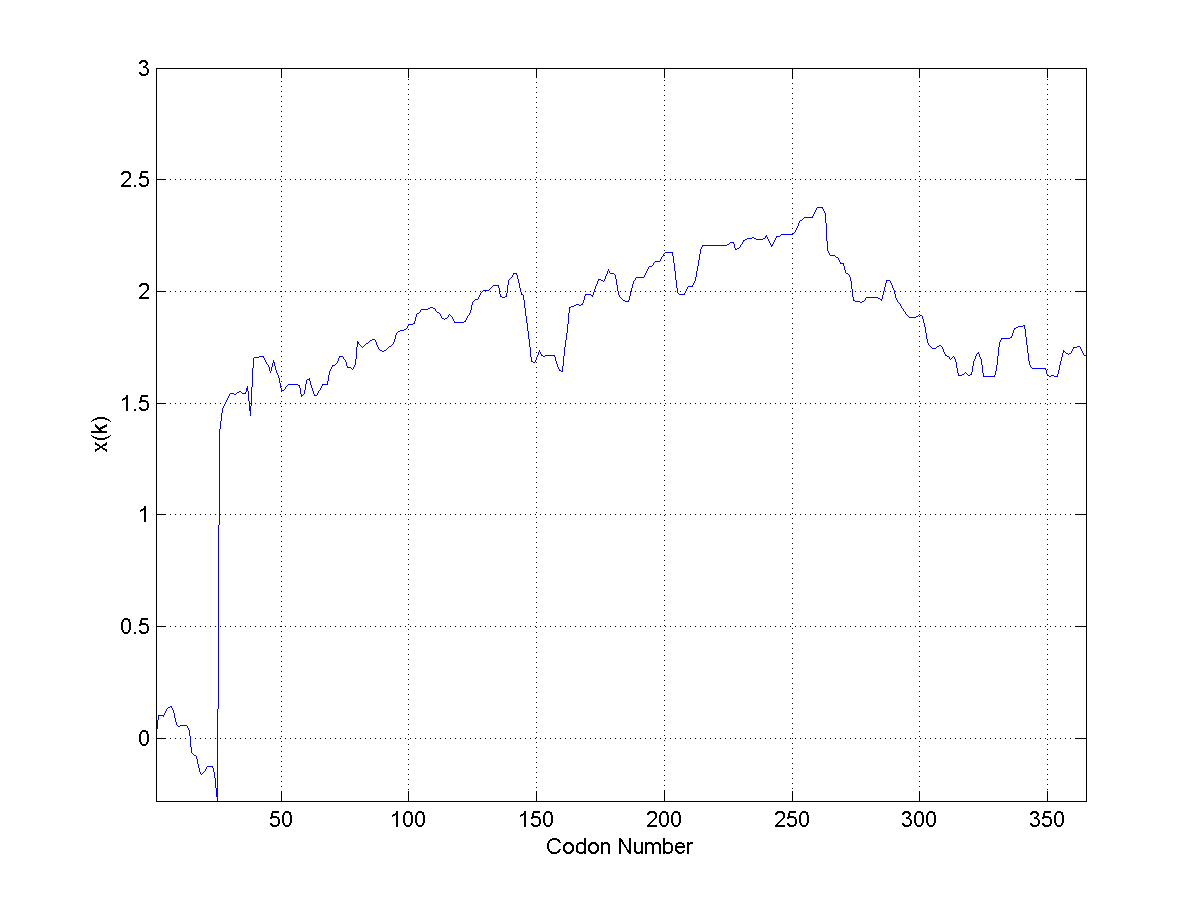
\includegraphics[scale=0.4]{prfB/disp}
\end{figure}

In \ecoli, the gene \prfB\ codes for protein release factor B, an
essential element in translation.  This gene, as mentioned, is known
to have a programmed frameshift at the 25$^{\textrm{th}}$ codon.  Our
proposed stochastic model, as with the original model, can accurately
predict this frameshift.  \autoref{prfB} shows a displacement plot for
\prfB, again with a distinctive jump at codon 25.  To account for
random variation, ten different runs are shown on the same set of
axes.
\footnote{Note that the polar plot is the the same as \autoref{prfB:polar}. 
The new model does not alter the polar plot or the free energy calculations.}

Notably, the displacement plot does not reach $x=2$ over the span of one codon, as the old model predicted.
Rather, due to randomness, the ribosome chooses the codon in the $+1$ frame before actually reaching a displacement of exactly 2.
The propensity to approach $x=2$, however, concurs with biological
evidence indicating the ribosome stays in frame after the frameshift.

For these plots, we used a species angle of $\theta_{\rm{sp}} =-30\degree$.
Yet, we must note that the model is quite robust; minor changes
in $\theta_{\rm{sp}}$ and initial displacement do not affect frameshifting significantly.
\autoref{prfB:sens} illustrates the error-free rate as
a function of species angle and initial displacement. As noted,
the frameshift holds over quite a wide range.

\subsection{Biological Verification for \prfB}
\begin{figure}
  \centering
  \caption{Sensitivity plot for \prfB}
  \label{prfB:sens}
  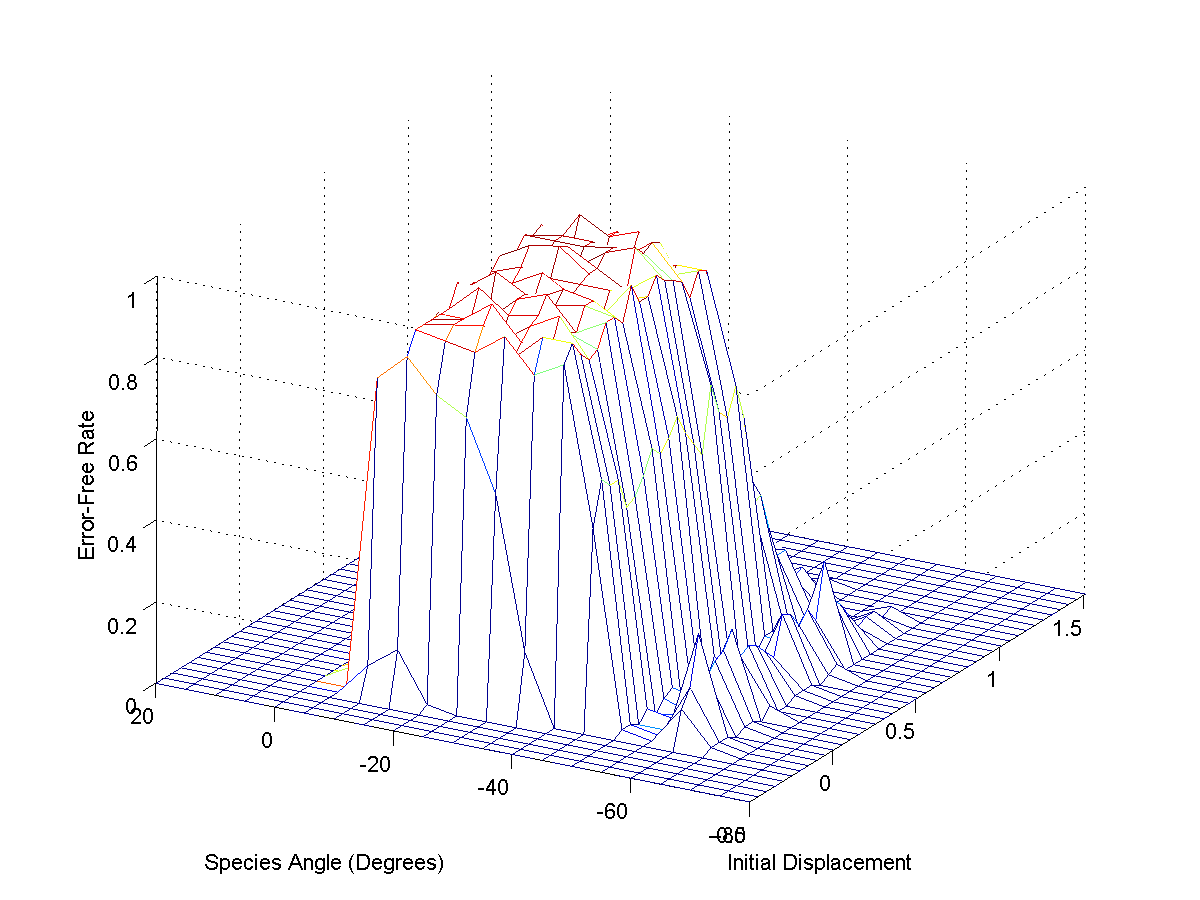
\includegraphics[scale=0.4]{prfB/sensitivity}
\end{figure}

\citet{weiss87,weiss88} conducted research on the
frameshift in \prfB, determining factors that would affect
translational rate.  We repeated Weiss's experiments computationally
using the stochastic model, and our results agreed.
This concurrence again provides support for the biological validity of
the stochastic model.

Specifically, \citeauthor{weiss87} moved the stop codon in the
\prfB\ sequence one nucleotide upstream, causing the sequence to fail to
frameshift. Moving the stop codon another nucleotide upstream failed
to create a frameshift as well. \autoref{prfb:weiss}
shows the displacement of these sequences.  As illustrated,
the frameshift is absent in both displacement plots at the proper codon.
The jump in the displacement later in the sequence may correspond to a
stop codon, or a sufficiently rare codon, that it encounters.

\begin{figure}
    \centering
    \caption{\prfB\ with Weiss's modifications}
    \label{prfb:weiss}
    \subfloat[One Base Pair]{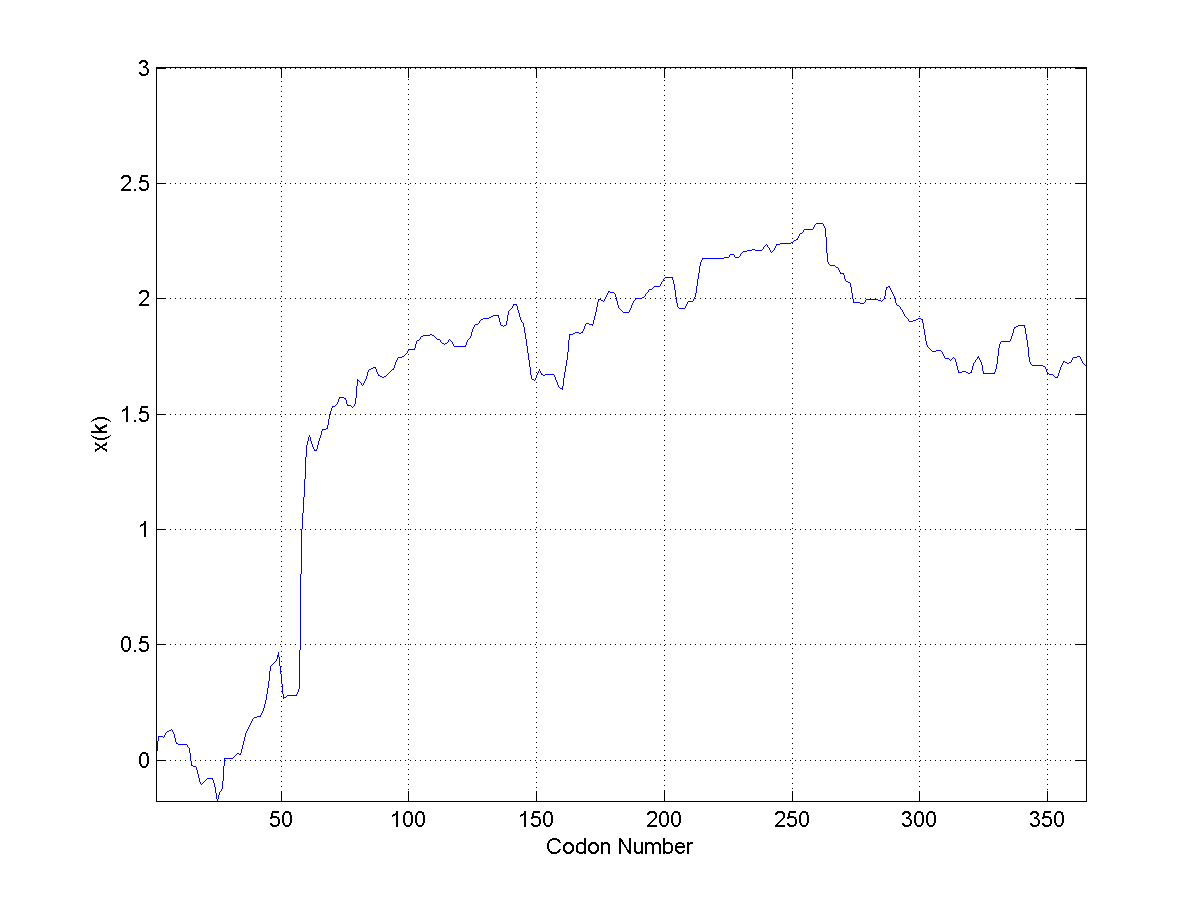
\includegraphics[scale=0.4]{prfb/weiss1}}
    \subfloat[Two Base Pairs]{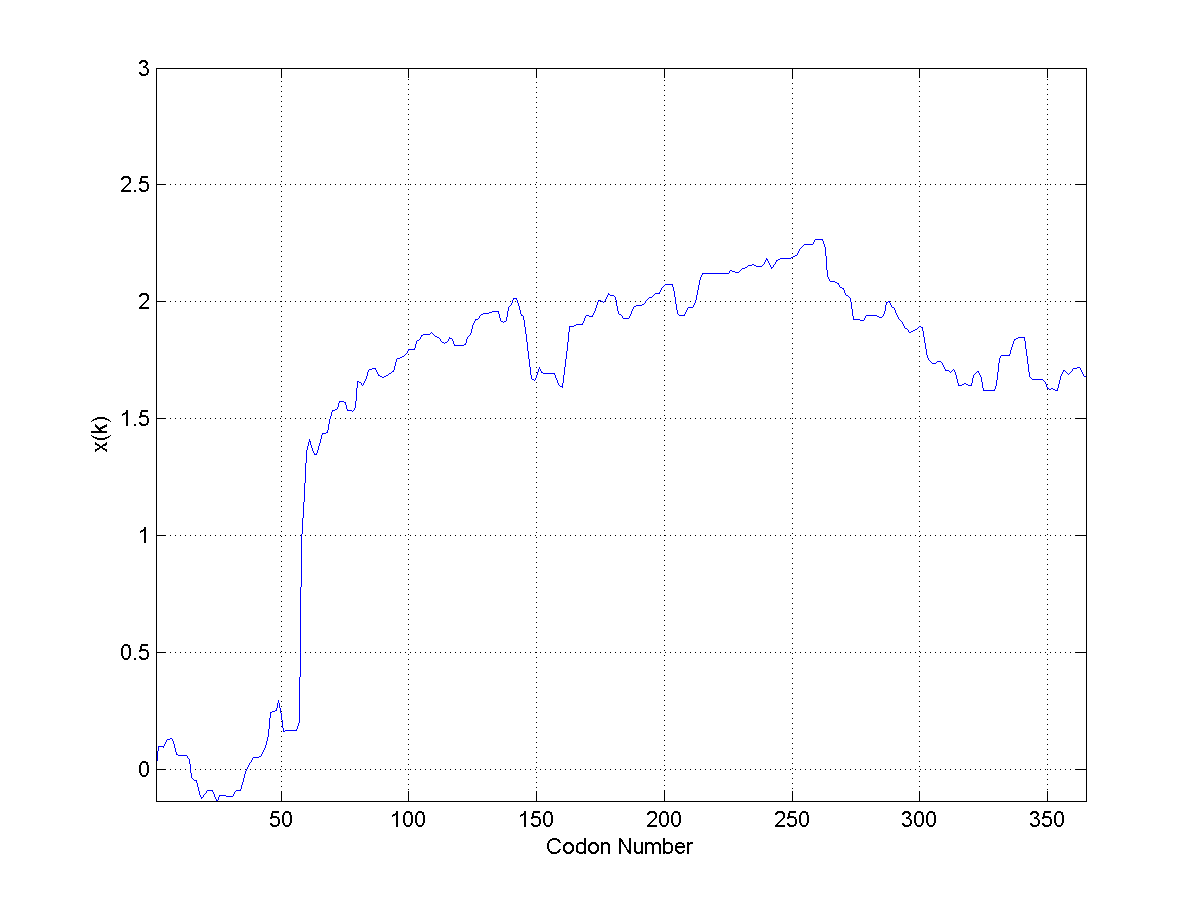
\includegraphics[scale=0.4]{prfb/weiss2}}
\end{figure}

In another experiment, \citeauthor{weiss88} altered the sequence of the
16S ribosomal tail, changing one nucleotide in the Shine-Dalgarno-like region
from guanine to cytosine.  As predicted by the stochastic model, this
change derailed the frameshift.

In all the cases discussed, 1000 iterations of the stochastic model
suggested that the sequence would frameshift at the desired location 0\%
of the time.  Although such a number is somewhat drastic by experimental
standards \cite{weiss87,weiss88}, it indicates that the model provides
strong predictive power.

\subsection{Verification: An Artificial Frameshifter}

\begin{figure}
  \centering
  \caption{Artificial linker sequence sensitivity plot}
  \label{linker:sens}
  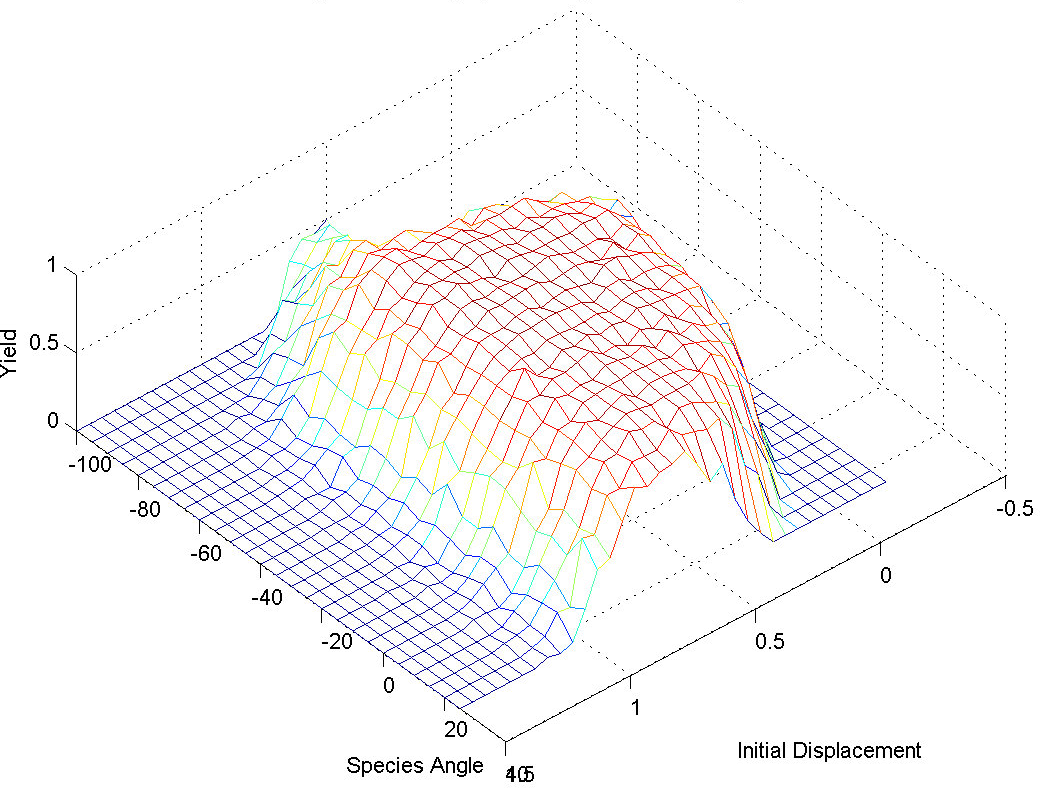
\includegraphics[scale=0.25]{linker/sensitivity}
\end{figure}

\begin{wrapfigure}{R}{0.55\textwidth}
  \caption{Artificial linker sequence}
  \label{linker}
  \begin{verbatim}
    aga aau cag acc
    aug gag gcu ggc acc
    agg ggg uac agu  u  aag caa acg
  \end{verbatim}
\end{wrapfigure}

In order to verify the model's ability to predict frameshifts, we
artificially created a sixteen-codon sequence (\autoref{linker})
designed to frameshift.  The sequence is designed to frameshift into
the \textsc{aag} frame after crossing the sole uracil.  Figure~\ref{linker:sens}
shows the error-free rate of the linker sequence as a function of species
angle and initial displacement, in order to demonstrate robustness,
similar to the \prfB\ sensitivity plot (\autoref{prfB:sens}).

A BLAST search finds about thirty matches of our sequence within areas of
bacterial genomes but none from \ecoli. To test the frameshifting capacity of
this linker sequence, we initiate a biological experiment.

We create a bifunctional fusion protein containing beta-galactosidase (\bgals) 
and \xylE.  Beta-galactosidase levels correlate to
levels of nitrophenol, which has a yellow color, while \xylE\ expresses
an enzyme that cleaves catechol.  These two proteins are joined by
the proposed linker sequence.  Research indicates that even in this
fused protein, both \bgals\ and \xylE\ should retain their functionalities.
As such, if the frameshift were to occur, one should observe both 
high levels of nitrophenol and low levels of catechol.

The biological construct for this experiment is in the process of being created.
Results should be available by mid-October.

\section{Conclusion}

As genetics becomes increasingly important in numerous fields, the
promise of mass-scale protein production remains one of the associated dreams.
Yet, the inescapable
component of biological experimentation remains a bottleneck that
presents time constraints and confounded data
alien to a fast-paced field with enormous potential. As such, an
accurate computational model is an invaluable tool. 
Our model provides a basis for a method of modeling ribosomal translation.
We have presented a metric for translational efficiency, running it on
ribosomal proteins, which likely have efficient translation rates.
More importantly, our work concurs with biological experiments dealing with bovine growth hormone,
accurately distinguishing between low-yield and high-yield proteins.
The model can also identify the programmed frameshift in \prfB,
and we used this capability to design an artificial sequence that we hypothesize to frameshift.

Although we have presented a large amount of circumstantial evidence
to support our model, we would like to test our theory on translational efficiency
on other gene sequences.  Sets of sequences known to be translationally regulated
can be run in the model to compare results to those found for bGH.
The genetic algorithm can be modified to account for larger sets of training
data.  Eventually, we hope to expand the model to account for other species of
bacteria using the same principles as the ones we used for \ecoli.

Our model provides a number of analytical tools of potential use to 
microbiologists designing synthetic gene sequences, a process used to
produce useful proteins for industry and medicine.
With the code publicly available, we hope to gather enough data over the
next few years to improve the accuracy of this model even further.
Our work thus represents an ongoing process that has the potential
to revolutionize biotechnology.

This model, including algorithms, is available as a collection of
Matlab and Perl scripts available on the Internet, open source and documented.

\addcontentsline{toc}{section}{References}
\begin{singlespace}
  \bibliography{wizards}
\end{singlespace}
\end{document}
